\begin{testproblem}
\label{test_prob:prob_v_quad_func}
\begin{gather}
\min_{x\in\R^2}\ (x_1 - 4)^2 + (x_2 - 7)^2 \notag \\
\begin{split}
\nb -10 \leq x_i & \leq 10,\ i = 1,2 \\
\end{split}
\end{gather}
\begin{equation*}
x^0 = (8, 9)^T \quad\text{und}\quad \xopt = (4, 7)^T.
\end{equation*}
\end{testproblem}

\begin{testproblem}
(Rosenbrock-Funktion, vgl. Beispiel 1.4.1 in \cite[S.~14]{alt})
\begin{gather}
\min_{x\in\R^2}\ 100 (x_2-x_1^2)^2+(1-x_1)^2  \notag \\
\begin{split}
\nb -10 \leq x_i & \leq 10,\ i = 1,2 \\
\end{split}
\end{gather}
\begin{equation*}
x^0 = (-1, 2)^T \quad\text{und}\quad \xopt = (1, 1)^T.
\end{equation*}
\end{testproblem}

\begin{figure}[h]
  \centering
  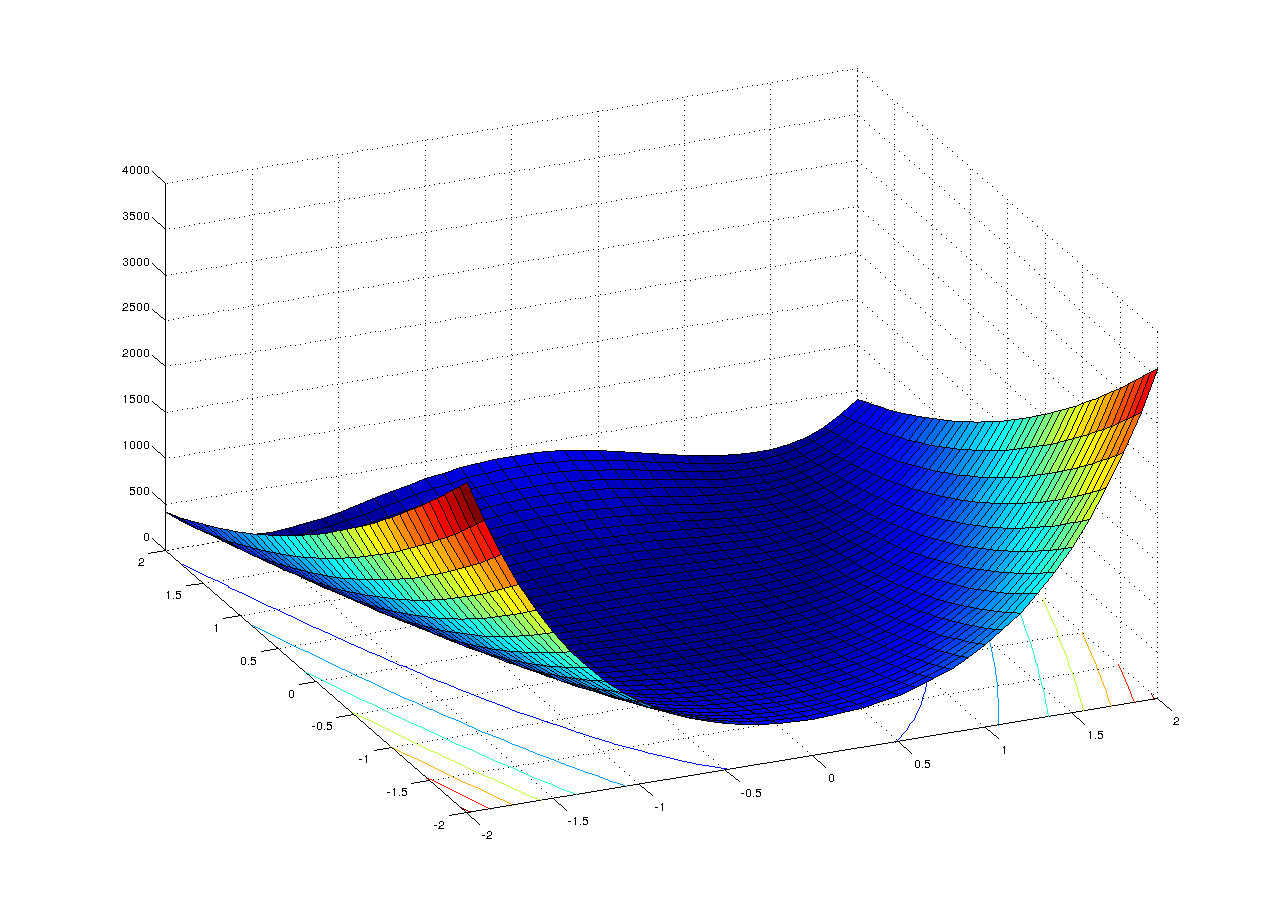
\includegraphics[width=0.45\textwidth]{rosenbrock}
  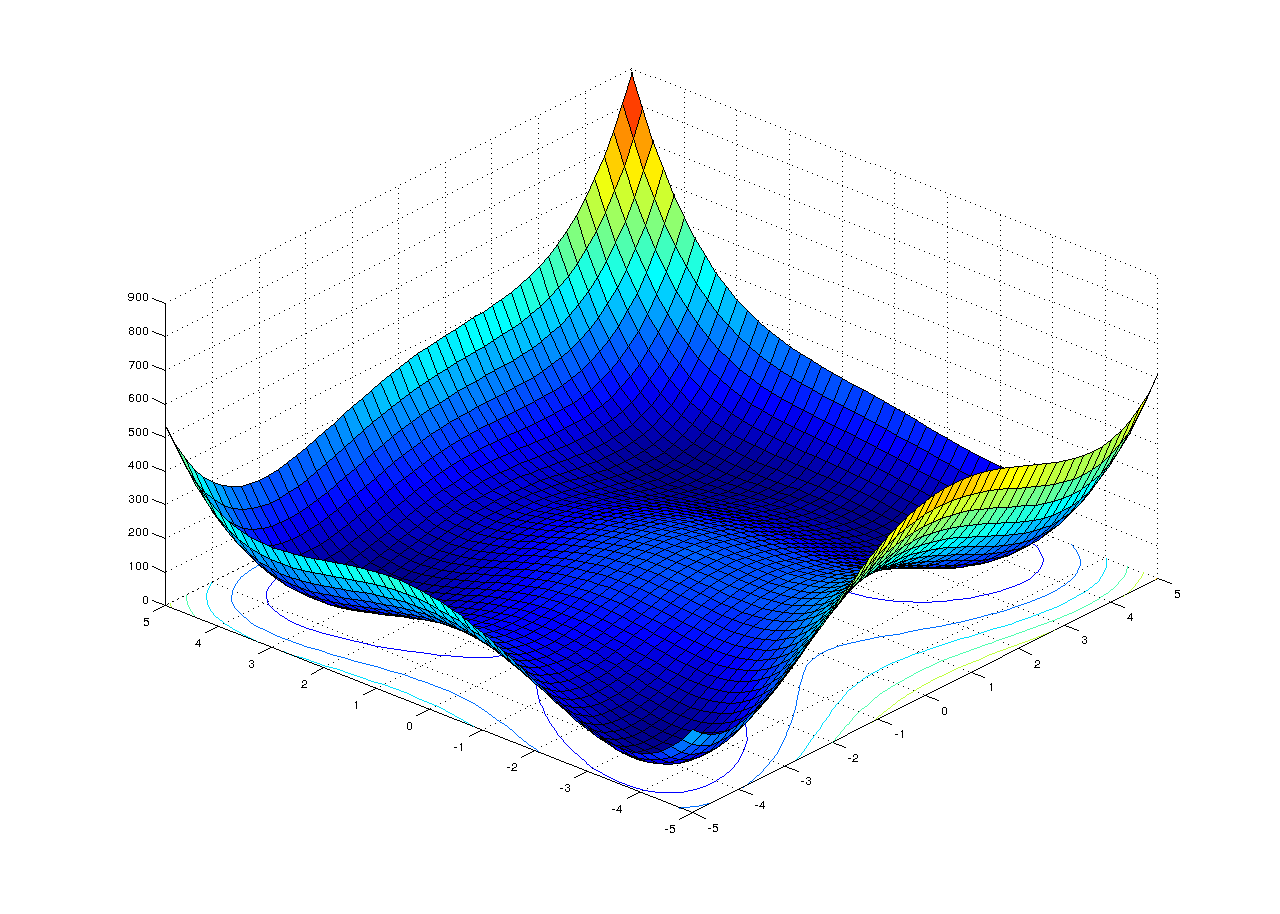
\includegraphics[width=0.45\textwidth]{himmelblau}
  \caption{Rosenbrock- und Himmelblau-Funktion}
  \label{fig:rosenbrock_und_himmelblau}
\end{figure}

\begin{testproblem}
(Himmelblau-Funktion, vgl. Beispiel 1.4.2 in \cite[S.~14~f.]{alt})
\begin{gather}
\min_{x\in\R^2}\ (x_1^2+x_2-11)^2 + (x_1+x_2^2-7)^2  \notag \\
\begin{split}
\nb -10 \leq x_i & \leq 10,\ i = 1,2 \\
\end{split}
\end{gather}
\begin{equation*}
x^0 = (5, 5)^T \quad\text{und}\quad \xopt = (3, 2)^T.
\end{equation*}
\end{testproblem}

\begin{testproblem}
(Bazaraa-Shetty-Funktion, vgl. Beispiel 1.4.3 in \cite[S.~15~f.]{alt})
\begin{gather}
\min_{x\in\R^2}\ (x_1-2)^4+(x_1-2 x_2)^2  \notag \\
\begin{split}
\nb -10 \leq x_i & \leq 10,\ i = 1,2 \\
\end{split}
\end{gather}
\begin{equation*}
x^0 = (5, 5)^T \quad\text{und}\quad \xopt = (2, 1)^T.
\end{equation*}
\end{testproblem}

\begin{testproblem}
(Beale-Funktion, vgl. Aufgabe 2.2 in \cite[S.~39]{alt})
\begin{gather}
\min_{x\in\R^2}\ (1.5-x_1 (1-x_2))^2+(2.25-x_1 (1-x_2^2))^2+(2.625-x_1 (1-x_2^3))^2  \notag \\
\begin{split}
\nb -10 \leq x_i & \leq 10,\ i = 1,2 \\
\end{split}
\end{gather}
\begin{equation*}
x^0 = (5, 0)^T \quad\text{und}\quad \xopt = (3, 0.5)^T.
\end{equation*}
\end{testproblem}

\begin{testproblem}
(Exponent-Funktion)
\begin{gather}
\min_{x\in\R^2}\ e^{\|x\|^2} \notag \\
\begin{split}
\nb -10 \leq x_i & \leq 10,\ i = 1,2 \\
\end{split}
\end{gather}
\begin{equation*}
x^0 = (5, 4)^T \quad\text{und}\quad \xopt = (0, 0)^T.
\end{equation*}
\end{testproblem}

\begin{figure}[h]
  \centering
  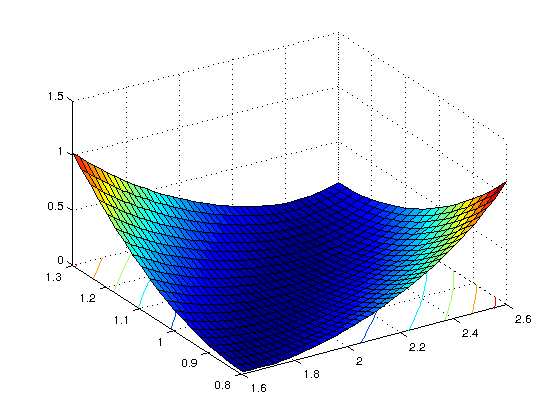
\includegraphics[width=0.45\textwidth]{bazaraa-shetty}
  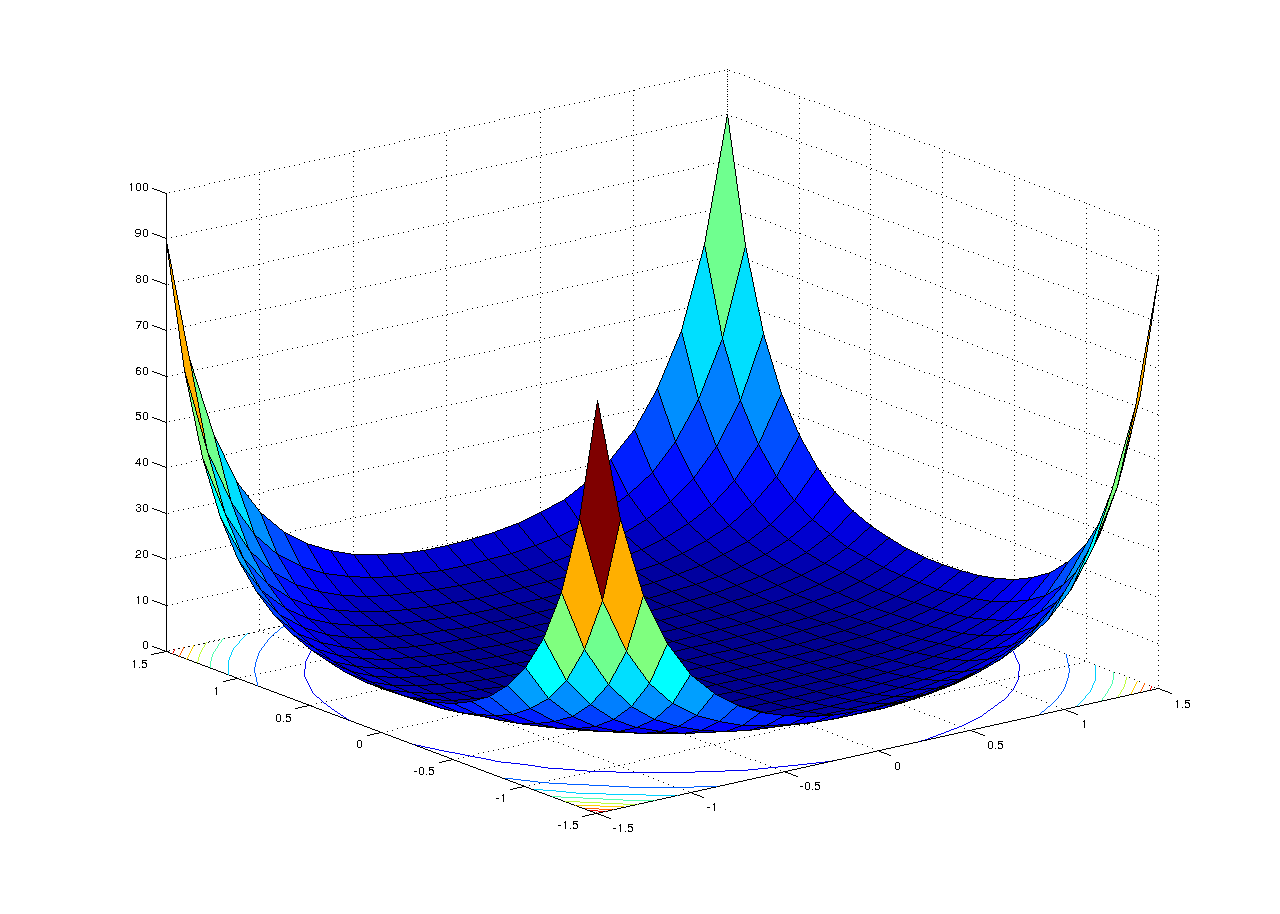
\includegraphics[width=0.45\textwidth]{exp-func}
  \caption{Bazaraa-Shetty- und Exponent-Funktion}
  \label{fig:bazaraa_shetty_und_exp_funktion}
\end{figure}

\begin{testproblem}
\begin{gather}
\begin{split}
  \min_{x\in\R^4}\ & 100(x_2-x_1^2)^2 + (1-x_1)^2 + 90(x_4-x_3^2)^2 + (1-x_3)^2\\
    & + 10.1((x_2-1)^2 + (x_4-1)^2) + 19.8(x_2-1)(x_4-1)
\end{split} \notag \\
\begin{split}
\nb -10 \leq x_i & \leq 10,\ i = 1,\ldots,4 \\
\end{split}
\end{gather}
\begin{equation*}
x^0 = (3, -1, -3, -1)^T \quad\text{und}\quad \xopt = (1, 1, 1, 1)^T.
\end{equation*}
\end{testproblem}

\begin{testproblem}
(Dixon-Funktion, vgl. Beispiel 1.4.5 in \cite[S.~16]{alt})
\begin{gather}
\min_{x\in\R^{10}}\ (1-x_1)^2 + \sum_{k=1}^{9} (x_k^2-x_{k+1})^2 + (1-x_{10})^2 \notag \\
\begin{split}
\nb -10 \leq x_i & \leq 10,\ i = 1,\ldots,10 \\
\end{split}
\end{gather}
\begin{equation*}
x^0 = (10, \ldots, 10)^T \quad\text{und}\quad \xopt = (1, \ldots, 1)^T.
\end{equation*}
\end{testproblem}

\begin{testproblem}
\begin{gather}
\min_{x\in\R^3}\ (x_1 - 4)^2 + (x_2 - 2)^2 + (x_3 - 7)^2 \notag \\
\begin{split}
\nb 5 \leq x_i & \leq 10,\ i = 1,2,3 \\
\end{split}
\end{gather}
\begin{equation*}
x^0 = (7, 10, 9)^T \quad\text{und}\quad \xopt = (5, 5, 7)^T.
\end{equation*}
\end{testproblem}

\begin{testproblem}
(Rosenbrock-Funktion)
\begin{gather}
\min_{x\in\R^2}\ 100 (x_2-x_1^2)^2+(1-x_1)^2  \notag \\
\begin{split}
\nb -10 \leq x_1 & \leq 10 \\
1.5 \leq x_2 & \leq 10 \\
\end{split}
\end{gather}
\begin{equation*}
x^0 = (2, 3)^T \quad\text{und}\quad \xopt = (1.224, 1.5)^T.
\end{equation*}
\end{testproblem}

\begin{testproblem}
(Himmelblau-Funktion)
\begin{gather}
\min_{x\in\R^2}\ (x_1^2+x_2-11)^2 + (x_1+x_2^2-7)^2  \notag \\
\begin{split}
\nb -10 \leq x_1 & \leq 10 \\
5 \leq x_2 & \leq 10 \\
\end{split}
\end{gather}
\begin{equation*}
x^0 = (10, 10)^T \quad\text{und}\quad \xopt = (-2.928, 5)^T.
\end{equation*}
\end{testproblem}

\begin{testproblem}
(Bazaraa-Shetty-Funktion)
\begin{gather}
\min_{x\in\R^2}\ (x_1-2)^4+(x_1-2 x_2)^2  \notag \\
\begin{split}
\nb 4 \leq x_1 & \leq 10 \\
-10 \leq x_2 & \leq 10 \\
\end{split}
\end{gather}
\begin{equation*}
x^0 = (7, 5)^T \quad\text{und}\quad \xopt = (4, 2)^T.
\end{equation*}
\end{testproblem}

\begin{testproblem}
\label{test_prob:prob_v_beale_1}
(Beale-Funktion)
\begin{gather}
\min_{x\in\R^2}\ (1.5-x_1 (1-x_2))^2+(2.25-x_1 (1-x_2^2))^2+(2.625-x_1 (1-x_2^3))^2  \notag \\
\begin{split}
\nb 3 \leq x_1 & \leq 10 \\
-10 \leq x_2 & \leq 10 \\
\end{split}
\end{gather}
\begin{equation*}
x^0 = (5, 0)^T \quad\text{und}\quad \xopt = (3, 0.5)^T.
\end{equation*}
\end{testproblem}

\begin{testproblem}
(Exponent-Funktion)
\begin{gather}
\min_{x\in\R^3}\ e^{\|x\|^2} \notag \\
\begin{split}
\nb 0.5 \leq x_1 & \leq 10 \\
1 \leq x_2 & \leq 10 \\
1 \leq x_3 & \leq 10 \\
\end{split}
\end{gather}
\begin{equation*}
x^0 = (5, 2, 4)^T \quad\text{und}\quad \xopt = (0.5, 1, 1)^T.
\end{equation*}
\end{testproblem}

\begin{testproblem}
\begin{gather}
\begin{split}
  \min_{x\in\R^4}\ & 100(x_2-x_1^2)^2 + (1-x_1)^2 + 90(x_4-x_3^2)^2 + (1-x_3)^2\\
    & + 10.1((x_2-1)^2 + (x_4-1)^2) + 19.8(x_2-1)(x_4-1)
\end{split} \notag \\
\begin{split}
\nb 2 \leq x_1 & \leq 10 \\
-10 \leq x_2 & \leq 10 \\
-10 \leq x_3 & \leq 10 \\
-10 \leq x_4 & \leq 10 \\
\end{split}
\end{gather}
\begin{equation*}
x^0 = (3, -1, -3, -1)^T \quad\text{und}\quad \xopt = (2, 3.831, 0.03, -0.178)^T.
\end{equation*}
\end{testproblem}

\begin{testproblem}
(Dixon-Funktion)
\begin{gather}
\min_{x\in\R^{10}}\ (1-x_1)^2 + \sum_{k=1}^{9} (x_k^2-x_{k+1})^2 + (1-x_{10})^2 \notag \\
\begin{split}
\nb 2 \leq x_i & \leq 10,\ i = 1,\ldots,10 \\
\end{split}
\end{gather}
\begin{equation*}
x^0 = (10, \ldots, 10)^T \quad\text{und}\quad \xopt = (2, \ldots, 2, 2.5)^T.
\end{equation*}
\end{testproblem}

\begin{testproblem}
\label{test_prob:lin_regres}
Lineare Regression (Vgl. Beispiel~\ref{example:lineare_regression}
auf Seite~\pageref{example:lineare_regression})
\begin{gather}
\min_{x\in\R^2}\ \sum_{i=1}^{10} (x_1 \xi_i + x_2 - \eta_i)^2 \notag \\
\begin{split}
\nb -10 \leq x_i & \leq 10,\ i = 1,2 \\
\end{split}
\end{gather}
\begin{equation*}
x^0 = (-10, 10)^T.
\end{equation*}

Die Messwerte $(\xi_i,\eta_i), i = 1,\ldots,10,$
sind in der Tabelle~\ref{tbl:messwerte_lin_regres}
zu finden.
\begin{equation*}
\xopt = (0.7, -4.3)^T
\quad \Rightarrow \quad
\tilde{\eta}(\xi) = 0.7\, \xi - 4.3 \,.
\end{equation*}
\end{testproblem}

\begin{table}[h]
\centering
\begin{tabular*}{0.8\linewidth}{@{\extracolsep{\fill}}c|cccccccccc}
  $\xi_i$ & 1 & 2 & 3 & 4 & 5 & 6 & 7 & 8 & 9 & 10 \\
  \midrule
  $\eta_i$ & $-0.5$ & $-2$ & $-3$ & $-3$ & $-2.5$
    & $-2$ & $-1$ & 1 & 3 & $5.5$ \\
\end{tabular*}
\caption{Messwerte f�r Testprobleme~\ref{test_prob:lin_regres}
und~\ref{test_prob:nichtlin_regres_quad}}
\label{tbl:messwerte_lin_regres}
\end{table}

\begin{testproblem}
\label{test_prob:nichtlin_regres_quad}
Nichtlineare Regression mit dem funktionalen
Zusammenhang~\eqref{eq:nichtlin_regres_quad_zusammenhang}
(Vgl. Beispiel~\ref{example:nichtlineare_regression}
auf Seite~\pageref{example:nichtlineare_regression})
\begin{gather}
\min_{x\in\R^3}\ \sum_{i=1}^{10} (x_1 (\xi_i -x_2)^2 + x_3 - \eta_i)^2 \notag \\
\begin{split}
\nb -10 \leq x_i & \leq 20,\ i = 1,2,3 \\
\end{split}
\end{gather}
\begin{equation*}
x^0 = (1, 3, -4)^T.
\end{equation*}

Die Messwerte
in der Tabelle~\ref{tbl:messwerte_lin_regres}
sind zu benutzen.
\begin{equation*}
\xopt = (0.242, 4.056, -2.955)^T
\quad \Rightarrow \quad
\hat{\eta}(\xi) = 0.242\, (\xi - 4.056)^2 - 2.955 \,.
\end{equation*}
\end{testproblem}

\begin{figure}[h]
\centering
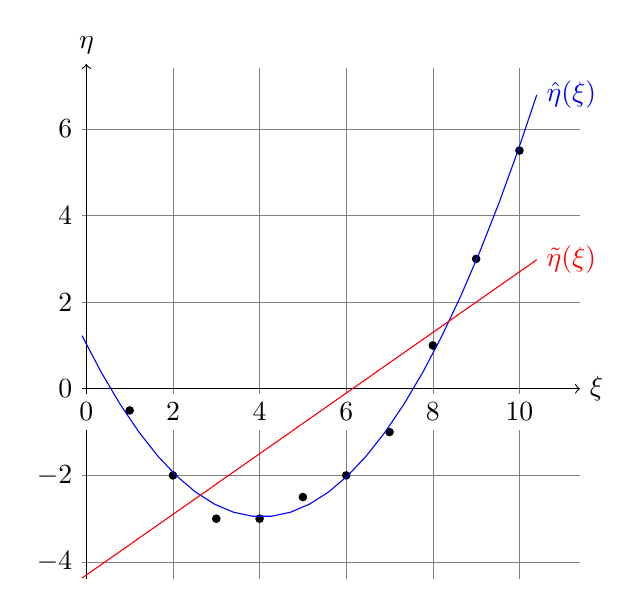
\begin{tikzpicture}[domain=-0.1:10.4,scale=0.55]
  \draw[very thin,color=gray,step=2] (-0.1,-4.4) grid (11.4,7.4);
  \draw[->] (-0.1,0) -- (11.4,0) node[right] {$\xi$};
  \draw[->] (0,-4.4) -- (0,7.5) node[above] {$\eta$};
  %\draw (-0.1,0.2) node [below left,fill=white] {0};
  \foreach \x in {0,2,4,...,10}
    \draw (\x,-0.1) node[below,fill=white] {$\x$};
  \foreach \y in {-4,-2,...,6}
    \draw (-0.1,\y) node[left] {$\y$};
  \foreach \x/\y in
    {1/-0.5, 2/-2, 3/-3, 4/-3, 5/-2.5, 6/-2, 7/-1, 8/1, 9/3, 10/5.5}
    \fill (\x,\y) circle(0.1);
  \draw[color=blue] plot (\x,{0.242*(\x-4.056)^2-2.955})
    node[right] {$\hat{\eta}(\xi)$};
  \draw[color=red] plot (\x,{0.7*\x-4.3})
    node[right] {$\tilde{\eta}(\xi)$};
\end{tikzpicture}
\caption{Ergebnisse der Testprobleme~\ref{test_prob:lin_regres}
und~\ref{test_prob:nichtlin_regres_quad}}
\end{figure}

\begin{testproblem}
\label{test_prob:nichtlin_regres_exp}
Nichtlineare Regression mit dem funktionalen
Zusammenhang~\eqref{eq:nichtlin_regres_exp_zusammenhang}
(Vgl. Beispiel~\ref{example:nichtlineare_regression}
auf Seite~\pageref{example:nichtlineare_regression})
\begin{gather}
\min_{x\in\R^2}\ \sum_{i=1}^{10} (x_1 e^{\xi x_2} - \eta_i)^2 \notag \\
\begin{split}
\nb -10 \leq x_i & \leq 10,\ i = 1,2 \\
\end{split}
\end{gather}
\begin{equation*}
x^0 = (0.2, 0.5)^T.
\end{equation*}

Die Messwerte $(\xi_i,\eta_i), i = 1,\ldots,10,$
sind in der Tabelle~\ref{tbl:messwerte_nichtlin_regres}
gegeben.
\begin{equation*}
\xopt = (0.632, 0.195)^T
\quad \Rightarrow \quad
\bar{\eta}(\xi) = 0.632\, e^{0.195\,\xi}.
\end{equation*}
\end{testproblem}

\begin{table}[h]
\centering
\begin{tabular*}{0.8\linewidth}{@{\extracolsep{\fill}}c|cccccccccc}
  $\xi_i$ & 1 & 2 & 3 & 4 & 5 & 6 & 7 & 8 & 9 & 10 \\
  \midrule
  $\eta_i$ & 1 & 1.1 & 1.2 & 1.35 & 1.55
    & 1.75 & 2.5 & 3 & 3.7 & 4.5 \\
\end{tabular*}
\caption{Messwerte f�r Testproblem~\ref{test_prob:nichtlin_regres_exp}}
\label{tbl:messwerte_nichtlin_regres}
\end{table}
